%% TeXora template: Motion Lab. Dark slides with cyan and magenta, and animations drawn with TikZ.
%% Every animation here is made with the animate package and plays in TeXora (and Adobe Acrobat).
%% Change the colours on the \definecolor lines below; the animations use them too.
% !TEX program = pdflatex
\documentclass[aspectratio=169]{beamer}
\usetheme{default}
\usepackage[T1]{fontenc}
\usepackage{lmodern}
\usepackage{tikz}
\usepackage{animate}
\definecolor{night}{RGB}{16,24,40}
\definecolor{panel}{RGB}{28,40,62}
\definecolor{glow}{RGB}{64,214,230}
\definecolor{spark}{RGB}{238,92,170}
\definecolor{mist}{RGB}{214,222,235}
\setbeamercolor{background canvas}{bg=night}
\setbeamercolor{normal text}{fg=mist}
\setbeamercolor{structure}{fg=glow}
\setbeamercolor{frametitle}{fg=glow}
\setbeamercolor{title}{fg=white}
\setbeamercolor{subtitle}{fg=glow}
\setbeamercolor{block title}{bg=panel,fg=glow}
\setbeamercolor{block body}{bg=panel!70!night,fg=mist}
\setbeamerfont{frametitle}{size=\Large,series=\bfseries}
\setbeamertemplate{navigation symbols}{}
\setbeamertemplate{blocks}[rounded]
\setbeamertemplate{itemize item}{\color{spark}$\bullet$}
\setbeamertemplate{footline}{%
  \hfill{\color{glow!60!night}\insertframenumber\,/\,\inserttotalframenumber}\hspace{1.2em}\vspace{0.8em}}
\setbeameroption{show notes on second screen=right}

\title{Motion Lab}
\subtitle{Slides that move}
\author{Your Name}
\institute{Your Institution}
\date{\today}

% A planet on its orbit, at angle #1 degrees.
\newcommand{\orbit}[1]{%
  \begin{tikzpicture}
    \draw[glow!35!night, line width=1pt] (0,0) circle (1.6);
    \fill[spark] (0,0) circle (0.28);
    \fill[glow] ({1.6*cos(#1)},{1.6*sin(#1)}) circle (0.14);
    \fill[glow!40!night] ({1.6*cos(#1-12)},{1.6*sin(#1-12)}) circle (0.09);
  \end{tikzpicture}}

\begin{document}

\begin{frame}
  \begin{columns}[c]
    \begin{column}{0.58\textwidth}
      {\usebeamercolor[fg]{title}\fontsize{30}{34}\selectfont\bfseries\inserttitle\par}
      \vspace{0.4em}
      {\usebeamercolor[fg]{subtitle}\Large\insertsubtitle\par}
      \vspace{1.6em}
      \insertauthor\par
      {\small\insertinstitute\par\insertdate\par}
    \end{column}
    \begin{column}{0.36\textwidth}
      \centering
      % Pulsing rings: plays as soon as the slide is shown, over and over.
      \begin{animateinline}[autoplay,loop]{12}
        \multiframe{24}{rR=0.2+0.06}{%
          
\begin{tikzpicture}
            \useasboundingbox (-1.8,-1.8) rectangle (1.8,1.8);
            \fill[spark] (0,0) circle (0.22);
            \draw[glow, line width=1.2pt] (0,0) circle (\rR);
            \draw[glow!50!night, line width=1pt] (0,0) circle ({\rR+0.5});
          \end{tikzpicture}}
      \end{animateinline}
    \end{column}
  \end{columns}
  \note{Welcome everyone. The rings move by themselves: this deck shows what animated slides can do.}
\end{frame}

\begin{frame}{Outline}
  \tableofcontents
  \note{Four kinds of motion: looping, back and forth, on a click, and at changing speeds.}
\end{frame}

\section{Looping}
\begin{frame}{An orbit that never stops}
  \begin{columns}[c]
    \begin{column}{0.45\textwidth}
      \centering
      \begin{animateinline}[autoplay,loop]{12}
        \multiframe{36}{rA=0+10}{\orbit{\rA}}
      \end{animateinline}
    \end{column}
    \begin{column}{0.5\textwidth}
      \begin{itemize}
        \item 36 pictures, 12 per second
        \item \texttt{autoplay}: starts when the slide is shown
        \item \texttt{loop}: begins again after the last picture
      \end{itemize}
    \end{column}
  \end{columns}
  \note{Let it run while you talk. Click it to pause and click again to carry on.}
\end{frame}

\begin{frame}{Back and forth}
  \centering
  % palindrome: plays forwards, then backwards, then forwards again.
  \begin{animateinline}[autoplay,palindrome]{20}
    \multiframe{20}{rA=-40+4}{%
      \begin{tikzpicture}
        \useasboundingbox (-2.4,-2.9) rectangle (2.4,0.3);
        \draw[mist!50!night, line width=1.5pt] (-1,0) -- (1,0);
        \draw[glow, line width=1.2pt] (0,0) -- ({2.4*sin(\rA)},{-2.4*cos(\rA)});
        \fill[spark] ({2.4*sin(\rA)},{-2.4*cos(\rA)}) circle (0.25);
      \end{tikzpicture}}
  \end{animateinline}
  \par\vspace{0.4em}
  A pendulum with \texttt{palindrome}: forwards, then backwards.
  \note{A palindrome animation never jumps back to the start; it swings back.}
\end{frame}

\begin{frame}{Two animations and a step}
  \begin{columns}[c]
    \begin{column}{0.45\textwidth}
      \centering
      \begin{animateinline}[autoplay,loop]{6}
        \multiframe{12}{rA=0+30}{%
          \begin{tikzpicture}
            \draw[glow!40!night, rounded corners] (-1.4,-1.4) rectangle (1.4,1.4);
            \draw[spark, line width=2pt, ->] (0,0) -- ({1.1*cos(\rA)},{1.1*sin(\rA)});
          \end{tikzpicture}}
      \end{animateinline}
    \end{column}
    \begin{column}{0.45\textwidth}
      \centering
      \begin{animateinline}[autoplay,loop,palindrome]{8}
        \multiframe{10}{iN=1+1}{%
          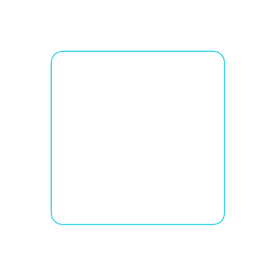
\begin{tikzpicture}
            \useasboundingbox (-1.4,-1.4) rectangle (1.4,1.4);
            \node[draw=glow, rounded corners, minimum size=2.2cm, font=\Huge\bfseries, text=glow] {\iN};
          \end{tikzpicture}}
      \end{animateinline}
    \end{column}
  \end{columns}
  \pause
  \vspace{0.6em}
  \begin{block}{On the next step}
    Animations keep playing while the points of a slide appear one by one.
  \end{block}
  \note{Press the right arrow once to show the block. Both animations go on.}
\end{frame}

\section{On a click}
\begin{frame}{Click to start}
  \centering
  % No autoplay: it waits. Click it, or use the buttons under it.
  \begin{animateinline}[controls]{12}
    \multiframe{24}{rA=0+15}{\orbit{\rA}}
  \end{animateinline}
  \par\vspace{0.3em}
  Without \texttt{autoplay} the animation waits for a click.
  \note{Click the animation when you are ready. TeXora's play, pause and step buttons sit under it on your screen.}
\end{frame}

\section{Speed}
\begin{frame}{Slow, then fast}
  \centering
  % Two pictures per second, then ten from the third picture on.
  \begin{animateinline}[autoplay,loop]{2}
    \tikz\node[draw=spark, line width=1.5pt, rounded corners, minimum size=2.4cm, font=\fontsize{40}{40}\selectfont, text=spark]{3};
    \newframe
    \tikz\node[draw=spark, line width=1.5pt, rounded corners, minimum size=2.4cm, font=\fontsize{40}{40}\selectfont, text=spark]{2};
    \newframe[10]
    \tikz\node[draw=glow, line width=1.5pt, rounded corners, minimum size=2.4cm, font=\fontsize{40}{40}\selectfont, text=glow]{1};
    \newframe
    \tikz\node[draw=glow, line width=1.5pt, rounded corners, minimum size=2.4cm, font=\fontsize{28}{28}\selectfont, text=glow]{Go};
  \end{animateinline}
  \par\vspace{0.4em}
  \texttt{\textbackslash newframe[10]} changes the speed in the middle.
  \note{The countdown starts slowly and speeds up.}
\end{frame}

\begin{frame}{Play once}
  \centering
  % autoplay without loop: plays once and stays on the last picture.
  \begin{animateinline}[autoplay]{15}
    \multiframe{30}{rW=0.2+0.2}{%
      
\begin{tikzpicture}
        \fill[panel, rounded corners] (0,0) rectangle (6,0.6);
        \fill[glow, rounded corners] (0,0) rectangle (\rW,0.6);
      \end{tikzpicture}}
  \end{animateinline}
  \par\vspace{0.6em}
  Without \texttt{loop} it plays once and stops on the last picture.
  \note{Good for a progress bar or a result that builds up once.}
\end{frame}

\begin{frame}{Summary}
  \begin{itemize}
    \item \texttt{autoplay}, \texttt{loop} and \texttt{palindrome} set how it plays
    \item Leave out \texttt{autoplay} to start it with a click
    \item \texttt{\textbackslash newframe[fps]} changes the speed
  \end{itemize}
  \vfill
  \begin{center}{\Large\color{glow} Thank you. Questions?}\end{center}
  \note{Thank the audience and invite questions.}
\end{frame}

\end{document}
